\documentclass[11pt,oneside, a4paper, titlepage]{article}
\usepackage{titlesec}
\usepackage{lipsum}
\usepackage{graphicx}
\usepackage{color}
\usepackage[nottoc]{tocbibind}
\usepackage[titletoc]{appendix}
\usepackage{amsthm}
\usepackage{titlesec}
\usepackage{tikz}
\usepackage{caption}
\usepackage{subcaption}
\usepackage[backend=bibtex, style=ieee, bibencoding=utf8]{biblatex}
\usepackage{amssymb}
\usepackage[utf8]{inputenc}
\usepackage[DIV=14,BCOR=2mm,headinclude=true,footinclude=false]{typearea}
\usepackage{csquotes}
\usepackage{todonotes}
\usepackage{hyperref}

\definecolor{keywordcolor}{rgb}{0.7, 0.1, 0.1}   % red
\definecolor{commentcolor}{rgb}{0.4, 0.4, 0.4}   % grey
\definecolor{symbolcolor}{rgb}{0.0, 0.1, 0.6}    % blue
\definecolor{sortcolor}{rgb}{0.1, 0.5, 0.1}      % green
\definecolor{background}{gray}{0.965}

\usepackage{listings}
\def\lstlanguagefiles{lstlean.tex}
\lstset{
  language=lean, 
  mathescape=true, 
  breaklines=true,
}
\newcommand{\dollar}{\mbox{\textdollar}}

\makeatletter
\DeclareCaptionFormat{alsoempty}{%
  #1\if\relax\expandafter\noexpand\lst@caption\else#2#3\fi}
\makeatother
\captionsetup[lstlisting]{format=alsoempty}

\newcommand\notes[1]{\textcolor{red}{#1}}

\theoremstyle{definition}
\newtheorem{definition}{Definition}[section]

\theoremstyle{definition}
\newtheorem{lemma}{Lemma}[section]

\addbibresource{refs.bib}

\newcommand\blfootnote[1]{%
  \begingroup
  \renewcommand\thefootnote{}\footnote{#1}%
  \addtocounter{footnote}{-1}%
  \endgroup
}

\newcommand{\sectionbreak}{\clearpage}

\begin{document}

% Title Page
\thispagestyle{empty}

\begin{center}

Vrije Universiteit Amsterdam

\vspace{1cm}


\includegraphics[height=28mm]{logo.png}

\vspace{1cm}

{\Large Bachelor Thesis}

\vspace*{1.5cm}

\rule{.9\linewidth}{.6pt}\\[0.4cm]
{\huge \bfseries Verifying AVL Trees\par}
{\huge \bfseries in Lean\par}\vspace{0.4cm}
\rule{.9\linewidth}{.6pt}\\[1.5cm]

\vspace*{2mm}

{\Large
\begin{tabular}{l}
{\bf Author:} ~~Sofia Konovalova ~~~~ (2635220)
\end{tabular}
}

\vspace*{1.5cm}

\begin{tabular}{ll}
{\it 1st supervisor:}   & ~~Jasmin Blanchette \\
{\it daily supervisor:} & ~~Jannis Limperg ~~~~ \\
{\it 2nd reader:}       & ~~Alexander Bentkamp
\end{tabular}

\vspace*{2cm}

\textit{A thesis submitted in fulfillment of the requirements for\\ the VU Bachelor of Science degree in Computer Science }

\vspace*{1cm}

\today\\[4cm] % Date

\end{center}

% \newenvironment{acknowledgements}%
%     {\cleardoublepage\thispagestyle{empty}\null\vfill\begin{center}%
%     \bfseries Acknowledgements\end{center}}%
%     {\vfill\null}
%         \begin{acknowledgements}
%           I would like to begin my thanking my daily supervisor, Jannis Limperg. You were incredibly helpful, patient and kind to me throughout this process, and it helped me build my confidence in a topic that was a completely new universe to me, and I would never have gotten this far without your encouragement. I would like to also thank all my friends who have been by my side as I was writing this thesis. Finally, I want to thank my parents who, even though they don't always fully understand, are still very supportful of me and my academic path.
%         \end{acknowledgements}

% \newpage

% \begin{abstract}
%   Using interactive theorem provers allow for researchers and mathematicians to create reusable formalized libraries of mathematics. This thesis contributes to this effort by creating a formalization of AVL trees. The AVL tree definitions and lemmas are outlined, with explanations of design changes made to fit Lean. Comparisons are made with existing definitions of red-black trees in Lean and AVL trees in other interactive theorem provers. Work is set to continue on the formalization, with changes made to make the proofs more efficient and remove overhead to integrate into the Lean mathlib library.
% \end{abstract}

\tableofcontents

\newpage

\section{Introduction}
In computer science, interactive theorem provers are used to develop formalizations of mathematical or logical concepts. The advantage of using these provers is that proofs can be long, or difficult to write by hand -- a good example is Fermat's Last Theorem, the full proof of which is known to be thousands of pages long. Additionally, there is no guarantee of the correctness of the initial proof statement. With interactive theorem provers, every proof step is verified by the lnaguage, which gives confidence in the correctness of the proof itself and the proof statement.

Interactive theorem provers, such as Coq, Isabelle and Lean, are used to develop formalizations of mathematical and logical concepts. Lean, though it is younger than Coq or Isabelle, already boasts mathlib \cite{The_mathlib_Community_2020}, a large library of formalized mathematics. Lean also improves on Coq by having a smaller kernel, cleaner syntax with Unicode support that can be written in Lean source files, and support for metaprogramming. 

Though matlib, through its detail and extensiveness has become a defacto standard library in Lean, is missing something, contrary to its counterparts Coq and Isabelle -- formalized tree structures. This thesis serves as a contribution to Lean and the mathlib library in the form of formalizing AVL trees, as well as a case study of the possibility of further formalization of search trees in Lean. 

The paper begins by giving a brief introduction to the Lean theorem prover, continuing on to a brief introduction on binary search trees and AVL trees, providing the corresponding Lean types and definitions. Afterwards, the verification process is discussed, proving all the necessary proof statements and changes made along the way. Finally, the formalization is compared to those made in Coq and Isabelle, and the future of this work is outlined.

\section{Lean Theorem Prover}
The Lean Theorem Prover is a proof assistant based on dependent type theory with inductive families and universal polymorphism \cite{inductive_families}. The language contains a hierarchy of universes, dependent function types and inductive types. This section will detail how these are outlined in the language.

In simple type theory, every expression has an associated type. Lean's dependent type theory extends simple type theory by having types themselves by types. Types can also be built from other types \cite{lean:manual}.  

\begin{lstlisting}
  universe u
  /- simple types -/
  constant m : nat
  constant b : bool
  /- types from other types -/
  constant g : nat → nat → nat
  #check g m -- nat → nat
\end{lstlisting}

With dependent type theory, types can depend on parameters. For example, \lstinline{list α} depends on \lstinline{α}, which helps differentiate between lists of different types. If we want to define a function which adds a new value to the list, the function would be polymorphic as its expected to function the same way with a \lstinline{bool}, \lstinline{nat} or any other \lstinline{α} type list. A function to add a new element to the list would have a type \lstinline{α → list α → list α}, which is an example of a dependent function type, as the outcome of the function is dependent on the type \lstinline{α} of the parameters.

In Lean, every type other than universes and every constructor other than a Pi is an instance of a family of type constructors are called inductive types \cite{lean:manual}. An inductive type is built from muliple constructors, and each constructor specifies a way of building some object. 

\begin{lstlisting}
inductive foo (a : α) : Sort u
| constructor₁: Π (b : β₁) → foo
| constructor₂: Π (b : β₂) → foo
\end{lstlisting}

An inductive type may be recursive if the arguments within the constructors \lstinline{(b₁ : β₁)} refer to the inductive type itself \cite{lean:reference}.


\section{AVL Trees and Operations}
AVL trees are a type of binary search trees (BSTs) that are self-balancing - meaning, it must be ordered and balanced after every operation. Balance and order is assumed and preserved by lookup, insertion and deletion. In Lean, the tree is implemented with an inductive type, and the operations are implemented as functions.

\subsection{Binary Search Trees}
\label{sec:bst}
A binary search tree (BST) (also called an ordered tree) is a tree data structure where each node has none, one, or two children. The children are referred to as the \textit{left child} and \textit{right child}. A node also has a key and a value for storing information.

Binary trees are defined as the following inductive type.

\begin{lstlisting}
inductive btree (α : Type u)
| empty {} : btree
| node (l : btree) (k : nat) (a : α) (r : btree) : btree
\end{lstlisting}

In this definition, there are two constructors: one for an empty tree and one for a node, with two children, a key (as a natural number) and a node value. There is no leaf constructor, as a leaf is a node with no children, which can be defined with the \lstinline{node} constructor.

From there, I defined a function to search for a key in a tree. The function verifies that a key exists in a tree; therefore, it doesn't matter in which subtree it is located in, as long as it is in one of them.

\begin{lstlisting}
def bound (x : nat) : btree α → bool
| btree.empty := ff
| (btree.node l k a r) :=
  x = k ∨ bound l ∨ bound r
\end{lstlisting}

A binary search tree must hold to the \textit{binary search property}.

\begin{definition}[Binary Search Property]
  \label{def:bst_property}
  Given any node N in a binary search tree, all the keys in the left subtree of N are smaller than the key of N, and all keys in the right subtree are greater than the 
  key of N.
\end{definition}

In Lean we define the binary search property with two separate definitions. The first one, \lstinline{forall_keys}, describes the relationship between a key and a tree -- for all the keys that exist in the tree, the relation \lstinline{nat → nat → Prop} holds for the input key and the keys in the tree.

\begin{lstlisting}
def forall_keys (p : nat → nat → Prop) (k : nat) (t : btree α) : Prop :=
  ∀ k', bound k' t → p k k'
\end{lstlisting}

The definition for \lstinline{ordered} formalizes the binary search property. A tree is ordered if the children are ordered and the \lstinline{forall_keys} relationship holds.

\begin{lstlisting}
def ordered : btree α → Prop
| btree.empty := tt
| (btree.node l k a r) :=
  ordered l ∧ ordered r ∧ (forall_keys (>) k l) ∧ (forall_keys (<) k r)
\end{lstlisting}

Due to the binary search property, lookup can be done recursively. For traversal, it is possible to compare every key to another as a total preorder is required for binary search trees. When traversing the tree, if the input key is smaller than the current node key, we recurse into the left subtree; if the input key is larger, we recurse into the right subtree.  

\begin{lstlisting}
def lookup (x : nat) : btree α → option α
| btree.empty := none
| (btree.node l k a r) :=
  if x < k then lookup l
  else if x > k then lookup r
  else a
\end{lstlisting}

\subsection{AVL Trees}
An AVL tree \cite{avl:original} is a self-balancing binary search tree, where the absolute value of the height difference between two child subtrees is no more than one.
This may also be described by the \textit{balancing factor}.

\begin{definition}[Tree height]
  \label{def:height}
  The height of a node in a tree is the maximal number of edges from that node to a leaf.
\end{definition}

\begin{definition}[Balancing factor]
  \label{def:balancing_factor}
  The balancing factor of any node is defined to be the height difference of its two child subtrees.
\end{definition}

In Lean, the definitions \lstinline{height} and \lstinline{balanced} are done per Definitions \ref{def:height} and \ref{def:bst_property}.

\begin{lstlisting}
def height : btree α → nat
| btree.empty := 0
| (btree.node l k a r) :=
  1 + (max (height l) (height r))

def balanced : btree α → bool
| btree.empty := tt
| (btree.node l k a r) :=
  if height l ≥ height r 
    then height l ≤ height r + 1
    else height r ≤ height l + 1
\end{lstlisting}

The process of looking up a node or searching for a key is the same as in BSTs. During insertion and deletion, however, a tree may become unbalanced, after which rotation algorithms are used to re-balance the tree. A tree can either be left-heavy or right-heavy. Left-heaviness can be fixed with a simple right rotation; right-heaviness with a simple left rotation. If the subtrees of the children are also unbalanced, compound rotations are used to re-balance, which consist of a right rotation followed by a left rotation or vice versa.

A tree \lstinline{t} being left-heavy means that if the right subtree has a height of $n$, the height of the left subtree is $n+2$; similarly, a right-heavy tree has a left subtree of height $n$ and a right subtree of height $n+2$. The definitions presented further closely follow \cite{textbook:discrete_computer}. The definition for \lstinline{right_heavy} is mirrored.

\begin{lstlisting}
def left_heavy : btree α → bool
| btree.empty := ff
| (btree.node btree.empty k a r) := ff
| (btree.node (btree.node ll lk la lr) k a r) :=
  (height ll ≥ height lr) ∧ (height ll ≤ height lr + 1) ∧
  (height lr ≥ height r) ∧ (height r + 1 = height ll)

def simple_right : btree α → btree α
| btree.empty := btree.empty
| (btree.node (btree.node ll lk la lr) k a r) := 
    btree.node ll lk la (btree.node lr k a r)
| (btree.node l k a r) := btree.node l k a r
\end{lstlisting}

\begin{figure}[!ht]
  \begin{subfigure}{0.5\textwidth}
    \centering
    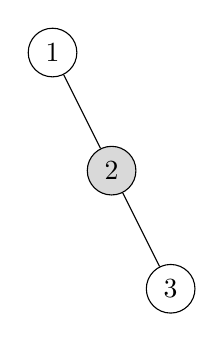
\begin{tikzpicture}
      \node[circle,draw](z){1}
        child[missing]{}
        child{
          node[circle,draw,fill=gray!30]{2} 
            child[missing] 
            child{
              node[circle,draw]{3}
              child[missing]
            }
          };
      \end{tikzpicture}
  \end{subfigure}%
  \begin{subfigure}{0.5\textwidth}
    \centering
    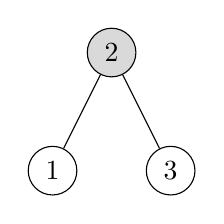
\begin{tikzpicture}
      \node[circle,draw,fill=gray!30](z){2}
        child{
          node[circle,draw]{1}
            child[missing]
            child[missing]
        }
        child{
          node[circle,draw]{3}
            child[missing]
            child[missing]
        };
    \end{tikzpicture}
  \end{subfigure}
  \label{fig:rotation}
  \caption{An example of a simple left rotation on a right-heavy tree.}
\end{figure}

In a simple right rotation, the pivot of the rotation is the left subtree, which is rotated. In a simple left rotation, the pivot of the rotation is the right subtree.

\begin{lstlisting}
def rotate_right : btree α → btree α
| btree.empty := btree.empty
| (btree.node l k a r) :=
  match l with
  | btree.empty := (btree.node l k a r)
  | (btree.node ll lk la lr) :=
    if height ll < height lr 
      then simple_right (btree.node (simple_left l) k a r)
      else simple_right (btree.node l k a r)
  end 
\end{lstlisting}

With simple rotations, only the height of the right (or left) child subtree matters. If the subtrees of the child are also too tall, i.e. too tall on the \enquote{inside}, a compound rotation needs to be applied. In the definition \lstinline{rotate_right}, the children of the left child are compared. If the left subtree of the child is smaller, a compound rotation is done as the tree is too heavy on the "inside". Otherwise, just a simple right rotation is done.

The insertion definition makes use of the definitions of heaviness and rotations to insert a node into a tree while retaining balance. If insertion creates a left-heavy tree, then a right rotation is done, and if it creates a right-heavy tree, then a left rotation is done.

\begin{lstlisting}
def insert (x : nat) (v : α) : btree α → btree α
| btree.empty := btree.node btree.empty x v btree.empty
| (btree.node l k a r) :=
  if x < k then 
    if left_heavy (insert l) 
      then rotate_right (btree.node (insert l) k a r)
      else btree.node (insert l) k a r
  else if x > k then
    if right_heavy (insert r) 
      then rotate_left (btree.node l k a (insert r))
      else btree.node l k a (insert r)
  else btree.node l x v r
\end{lstlisting}

Deletion is more complicated, and depends on the placement of the node within the tree. If the left subtree is empty, then the node can be safely replaced by the right subtree.  If the left subtree has children, it can be of any height, so re-balancing has to be taken into account. In this case, the same philosophy can be followed as for deletion when the left subtree is empty, but traveling down the right subtree and looking for an empty right child. If a node \lstinline{n} is found with an empty right child, the key and data value of \lstinline{n} is returned, and \lstinline{n} is replaced by its left child subtree, with right rotations performed to restore balance. 

\begin{lstlisting}[escapeinside={*}{*}]
def shrink : btree α → option (nat × α × btree α)
| btree.empty := none
| (btree.node l k v r) := some *\$*
  match shrink r with
  | none := (k, v, l)
  | some (x, a, sh) :=
    if height l > height sh + 1
      then (x, a, rotate_right (btree.node l k v sh))
      else (x, a, btree.node l k v sh)
  end
\end{lstlisting}

Since shrinking an empty tree is impossible, \lstinline{shrink} returns an \lstinline{option}.

The next step is to define the steps to delete a node. This is done with the function \lstinline{del_node}. If the left subtree of the node to be deleted is not empty, then the left subtree is shrunken, and a new tree is formed with the resulting key from the shrink operation as the new node, the shrunken tree and the original right subtree. A rotation is done if the result is unbalanced. 

\begin{lstlisting}
def del_node : btree α → btree α
| btree.empty := btree.empty
| (btree.node l k v r) :=
  match shrink l with 
  | none := r
  | some (x, a, sh) :=
    if height r > height sh + 1 then rotate_left (node sh x a r)
    else node sh x a r
  end
\end{lstlisting}

Finally, the full \lstinline{delete} function is complete. 

\begin{lstlisting}
def delete (x : nat) : btree α → btree α
| btree.empty := btree.empty
| (btree.node l k a r) :=
  let dl := delete l in
  let dr := delete r in
  if x = k then del_node (btree.node l k a r)
  else if x < k then
    if height r > height dl + 1 then rotate_left (btree.node dl k a r)
    else btree.node dl k a r
  else if height l > height dr + 1 then rotate_right (btree.node l k a dr)
  else (btree.node l k a dr)
\end{lstlisting}

First, find the node to delete. If it is found, then the \lstinline{del_node} function is called on the entire subtree. During the search of the node to delete, the operation is called recursively, and rotations are applied if the tree becomes unbalanced. 

\section{Verification}
In this section, we verify the operations presented above. Each subsection details examples of proof statements for specific operations and informally explains how to complete the proofs. AVL tree operations need to restore balance, as well as preserve order and keys. This section does not detail all of the proof constructions, but goes give all the necessary lemmas and proofs are detailed when it is either important to understand the proof statement or when the proof construction led to core design decisions. The lemma statements presented here closely follow \cite{textbook:discrete_computer}, though some changes were made to statements to suit the Lean definitions.

\subsection{BST Operations}
First, we prove two lemmas related to boundedness and lookup in a tree, since \lstinline{lookup} and \lstinline{bound} are identical for both BSTs and AVL trees.

\begin{lstlisting}
lemma bound_false (k : nat) (t : btree α) :
  bound k t = ff → lookup k t = none := ...

lemma bound_lookup (k : nat) (t : btree α) :
  ordered t → bound k t → ∃ (v : α), lookup k t = some v := ...
\end{lstlisting}

The lemma \lstinline{bound_false} states that if a key is not bound in a tree, then lookup will not result in any node data being returned. The lemma \lstinline{bound_lookup} states that if a key is bound in a tree, then some data will be returned. The existential quantifier is used in this lemma, because we cannot make assumptions on which key will return which value. In other words, we don't know the specific node value, but we do know that something will be returned. Both of the proofs were constructed by induction on the tree \lstinline{t}.

\subsection{Rotation}
With rotations we want to prove that an ordered tree preserves order after a rotation, and that if a tree is imbalanced then a rotation restores its balance. This section will present two proofs on right rotations preserving order and balance.

\subsection*{Order}
\begin{lstlisting}[caption=\empty, label={lst:right_ordered}]
lemma rotate_right_ordered (t : btree α) :
  ordered t → ordered (rotate_right t) := ...
\end{lstlisting}

Listing \ref{lst:right_ordered} shows a formalized lemma statement for right rotations preserving order. The first step with proof statements with rotations is to look at their definitions. The definition for \lstinline{rotate_right} uses the \lstinline{simple_right} and \lstinline{simple_left} definitions, so proofs about them preserving order need to be constructed too.

\begin{lstlisting}[caption=\empty, label={lst:simple_ordered}]
lemma simple_right_ordered (t : btree α) :
  ordered t → ordered (simple_right t) := ...

lemma simple_left_ordered (t : btree α) :
  ordered t → ordered (simple_left t) := ...
\end{lstlisting}

The proof in Listing \ref{lst:right_ordered} were done by case splitting on the tree \lstinline{t}, its right subtree \lstinline{r} and the next subtree \lstinline{lr}, and the simple rotation lemmas were applied throughout when needed. The simple rotation lemmas were also completed by case splitting on left or right subtree depending on the rotation.

The proofs above also require a lemma for transitivity of keys in trees. Assume a tree \lstinline{rr} and \lstinline{rl}, with the former having a left and a right child \lstinline{rll} and \lstinline{rlr}. Also assume two keys \lstinline{rk}, which is the parent node key of \lstinline{rr}, and \lstinline{rlk}, which is the key of \lstinline{rl}.
If \lstinline{rk} is greater than all the keys contained in \lstinline{rll} and \lstinline{rlr}, and \lstinline{rk} is less than the keys in \lstinline{rr}, by transitivity \lstinline{rlk} is less than all the keys in \lstinline{rr}. The lemma for key transitivity is formalized below.

\begin{lstlisting}[caption=\empty]
lemma forall_keys_trans (t : btree α) (p : nat → nat → Prop) 
(z x : nat) (h₁ : p x z) (h₂ : ∀ a b c, p a b → p b c → p a c) :
  forall_keys p z t → forall_keys p x t := ...
\end{lstlisting}

Another lemma had to be made to make constructing proofs with \lstinline{forall_keys} much easier. The current definition for \lstinline{forall_keys} does not take into consideration the relationship of the input key between the left and right children of the tree. The \lstinline{forall_keys_intro} introduction lemma solved this problem.

\begin{lstlisting}[caption=\empty]
lemma forall_keys_intro {l r : btree α} {k x : nat} {v : α} 
  {p : nat → nat → Prop} :
(forall_keys p k l ∧ p k x ∧ forall_keys p k r) 
  → forall_keys p k (node l x v r) := ...
\end{lstlisting}

When applying the introduction lemma, I was able to get the relation of the key between the left and right subtree, and the relation between the input key and the key of the tree, which made applying the transitivity lemma a lot easier.

\subsection*{Balance}

\subsection{Insertion}
Proofs about insertion into AVL trees, like the ones for rotation, need to show a preservation of order, keys, and balance restoration.

\subsection{Deletion}
This section will go through the proof construction of deletion preserving order, and the sub-proofs that come along with it as well as major changes that have been done to previous definitions to make the proof constructions easier and readable.

The lemma statement for deletion preserving order is formalized below.

\begin{lstlisting}[caption=\empty]
lemma delete_ordered (t : btree α) (k : nat) :
  ordered t → ordered (delete k t) :=
\end{lstlisting}

Since the function \lstinline{delete} uses \lstinline{del_node}, a similar proof has to be constructed for it as well. The lemma statement does not contain a key, as with \lstinline{del_node}, the tree is assumed to have the root that matches the key in the arguments of \lstinline{delete}.

\begin{lstlisting}[caption=\empty]
lemma del_node_ordered (t : btree α) (k : nat) :
  ordered t → ordered (del_node t) :=
\end{lstlisting}

Both of the above proofs were constructed by induction on the tree \lstinline{t}.

Since \lstinline{del_node} uses \lstinline{shrink}, a proof for \lstinline{shrink} preserving order needs to be constructed as well. The lemma statement needs to have the reuslt of \lstinline{shrink} as one of its hypotheses, and the conclusion is that the result of shrinking a tree is also ordered, and that the resulting key is larger than the keys in the shrunken tree.

\begin{lstlisting}[caption=\empty, label={lst:shrink_ordered}]
lemma shrink_ordered {t sh : btree α} {x : nat} {a : α} :
  ordered t ∧ shrink t = some (x, a, sh) → ordered sh ∧ forall_keys gt x sh :=
\end{lstlisting}

The proof for \lstinline{shrink_ordered} was done by induction on the tree, but generalizing \lstinline{x}, \lstinline{a} and \lstinline{sh}. This is because without the generalization, the proof would be referring to a specific result of \lstinline{shrink}, which cannot be foreseen, so therefore the proof needs to take into account all the possible values for the three-tuple result of \lstinline{shrink}.

During the proof, I came across a sitation where some of the hypotheses were about \lstinline{shrink}, but no information could be derived from them. This led to the creation of a view\footnote{\notes{write how this was done by the supervisor but idk how yet}} for \lstinline{shrink}, to show each possible variation of arguments for \lstinline{shrink} and the result that gives.

\begin{lstlisting}[caption=\empty]
inductive shrink_view {α} : btree α → option (nat × α × btree α) → Sort*
| empty : shrink_view empty none
| nonempty_empty : ∀ {l k v r},
  shrink r = none →
  shrink_view (node l k v r) (some (k, v, l))
| nonempty_nonempty₁ : ∀ {l k v r x a sh out},
  shrink r = some (x, a, sh) →
  height l > height sh + 1 →
  out = some (x, a, rotate_right (btree.node l k v sh)) →
  shrink_view (node l k v r) out
| nonempty_nonempty₂ : ∀ {l k v r x a sh},
  shrink r = some (x, a, sh) →
  height l ≤ height sh + 1 →
  shrink_view (node l k v r) (some (x, a, node l k v sh))
\end{lstlisting}

A lemma was also written for \lstinline{shrink_view}, that would result in case splits for each case in the view. 

\begin{lstlisting}[caption=\empty, label={lst:shrink_view}]
lemma shrink_shrink_view (t : btree α) : 
  shrink_view t (shrink t) :=
\end{lstlisting}

Applying the lemma shown in Listing \ref{lst:shrink_view} would result in three cases in the inductive step of the proof in Listing \ref{lst:shrink_ordered}.

\section{Related Work}
Formalizations of AVL trees, as well as other search trees, are present in both the Coq \cite{code:coq_avl} and Isabelle/HOL \cite{isabelle} interactive theorem provers. Lean does not have an AVL tree formalization yet, and the only other tree present int he mathlib library is a red-black tree. 

\subsection*{Coq}
In contrast to my approach, the Coq formalization has one single balance function, \lstinline{bal}, and no abstraction into separate left/right rotations. This can be seen as a stylistic choice, but it creates a very long definition and longer, more complicated proofs. While in my approach, the proofs are still relatively long, because lemmas are written for separate rotations, they can be applied to the long proof. It can have an effect on performance. The \lstinline{bal} function is used in insertion, which is recursive. My approach to the \lstinline{insert} function is to first determine whether it will result in a left- or right-heavy tree, and then rotate the tree after insertion, which saves operational time on not balancing a tree when it is not necessary.  

The definition of binary search trees in Coq and Lean are similar, the only difference is that height is included in the definition of trees in Coq, while in Lean height is calculated when needed. While this can be a stylistic choice, it may have an effect on performance. With every new node added, one is added to the height of each ancestor, while with the Lean interpretation height is calculated on demand, which takes longer the bigger the tree is.

\subsection*{Isabelle}
In the Isabelle formalization, are two functions \lstinline{balL} that re-balances left subtrees and \lstinline{balR} that re-balances right subtrees. They function similarly to \lstinline{rotate_right} and \lstinline{rotate_left}, and are used in the balancing function, which makes proofs more modular. Like in Coq, the height of the tree is included in the tree definitions.

\subsection*{Other Search Trees}
Isabelle/HOL has a libary of data structures, which apart from containing an AVL tree formalization, has other tree formalizations like red-black trees, 2-3 trees, and standard binary trees. In Coq, finite sets are implemented using AVL trees and red-black trees, which so far are the only trees present in the standard library. A generic binary search tree structure is also present that is used by both AVL and red-black tree definitions.

Lean itself has an inductive datatype \lstinline{bin_tree}, but no operations related to it. The mathlib library \cite{The_mathlib_Community_2020}, a standard library in Lean, has an inductive type \lstinline{tree} which is similar to \lstinline{btree}. Both of the definitions do not contain a key value in the type constructors, so as is, they cannot be used to create search trees, or create maps or sets. Red-black trees have definitions for the inductive type \lstinline{rbnode} and some definitions, but it is not completely formalized. 

\section{Conclusion}
Theorem provers such as Lean are used to create libraries of mathematics and logic, to be used for research and teaching. In this thesis, I presented a formalization of AVL search trees using Lean. Lean proof constructions a relatively simple and mechanical task, once the main hurdle of learning and getting used to the syntax. Overall, the proof statements presented in Lean were not very different to those presented informally in \cite{textbook:discrete_computer}, although some very small changes did have to be made. Additionally, definitions regarding the structure of AVL treees such as \lstinline{balance} and \lstinline{height} stay true to their mathematical definitions for trees. Hopefully, in the future, formalization of search trees as a form of contribution to mathematical libraries in Lean can continue and other abstract data structures may be formalized as well.

\subsection*{Further Work}
The continuation of this work would begin by completing proofs for insertion and deletion that are missing from the source code, for which the only cause is a lack of time. The next steps are to make use of Lean's automation and metaprogramming to create shorter and cleaner code, as well as improving definitions to remove overhead. The final step is the inclusion of this final formalization into the mathlib library.

\newpage

\printbibliography[heading=bibintoc]
\addtocontents{toc}{\protect\blfootnote{The full code presented this this thesis may be found at the following link: \url{https://github.com/reglayass/lean-thesis}}}

\end{document}
